\chapter{Конструкторская часть}
\label{cha:design}

В данной части будут приведены схемы алгоритмов Левенштейна в рекурсивной и матричной реализации и Дамерау-Левенштейна.

\section{Разработка алгоритмов}
% сюда схемы алгоритмов

Далее указаны разработанные схемы алгоритмов Левенштейна и Дамерау-Левенштейна.
Будем считать, что известны следующие функции:
определения длины строки,
поиска максимума и минимума среди нескольких чисел.
Для матричных реализаций требуется наличие функции, динамически выделяющей память.

На рис. \ref{levenshtein-recursive-scheme} представлена схема алгоритма определения расстояния Левенштейна в рекурсивной реализации.

\begin{figure}
    \centering
    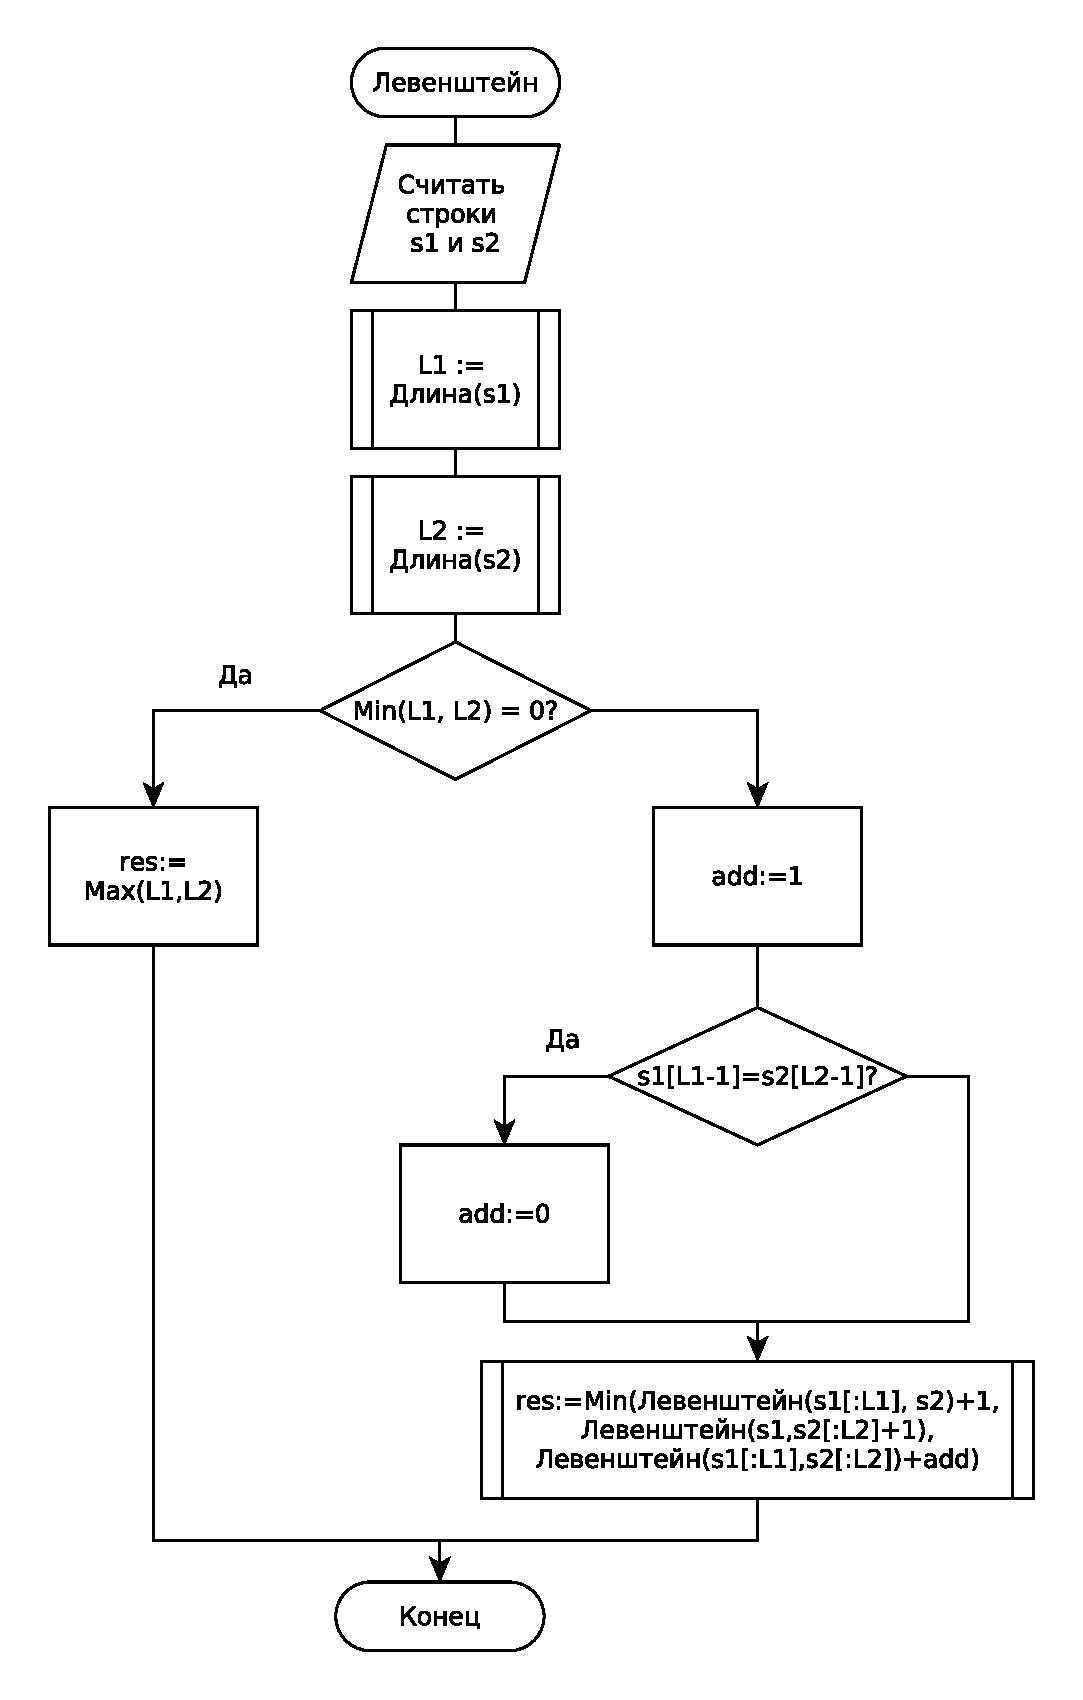
\includegraphics[height=0.75\textheight]{schemes/levenshtein-recursive-eps}
    \caption{Схема алгоритма определения расстояния Левенштейна в рекурсивной реализации.}
    \label{levenshtein-recursive-scheme}
\end{figure}

\FloatBarrier

На рис. \ref{levenshtein-iterative-scheme-part-1} и на рис. \ref{levenshtein-iterative-scheme-part-2} представлена 1 часть схемы алгоритма определения расстояния Левенштейна в матричной реализации.

\begin{figure}
    \centering
    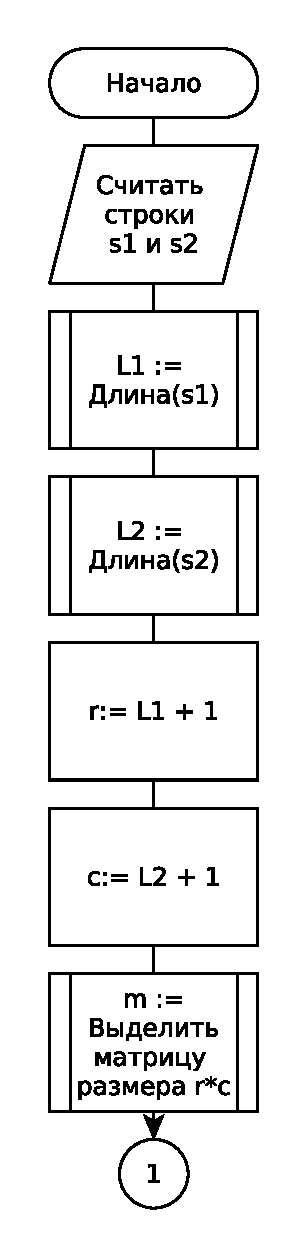
\includegraphics[height=0.75\textheight]{schemes/levenshtein-iterative-eps-1}
    \caption{Схема алгоритма определения расстояния Левенштейна в матричной реализации. Часть 1.}
    \label{levenshtein-iterative-scheme-part-1}
\end{figure}

\begin{figure}
    \centering
    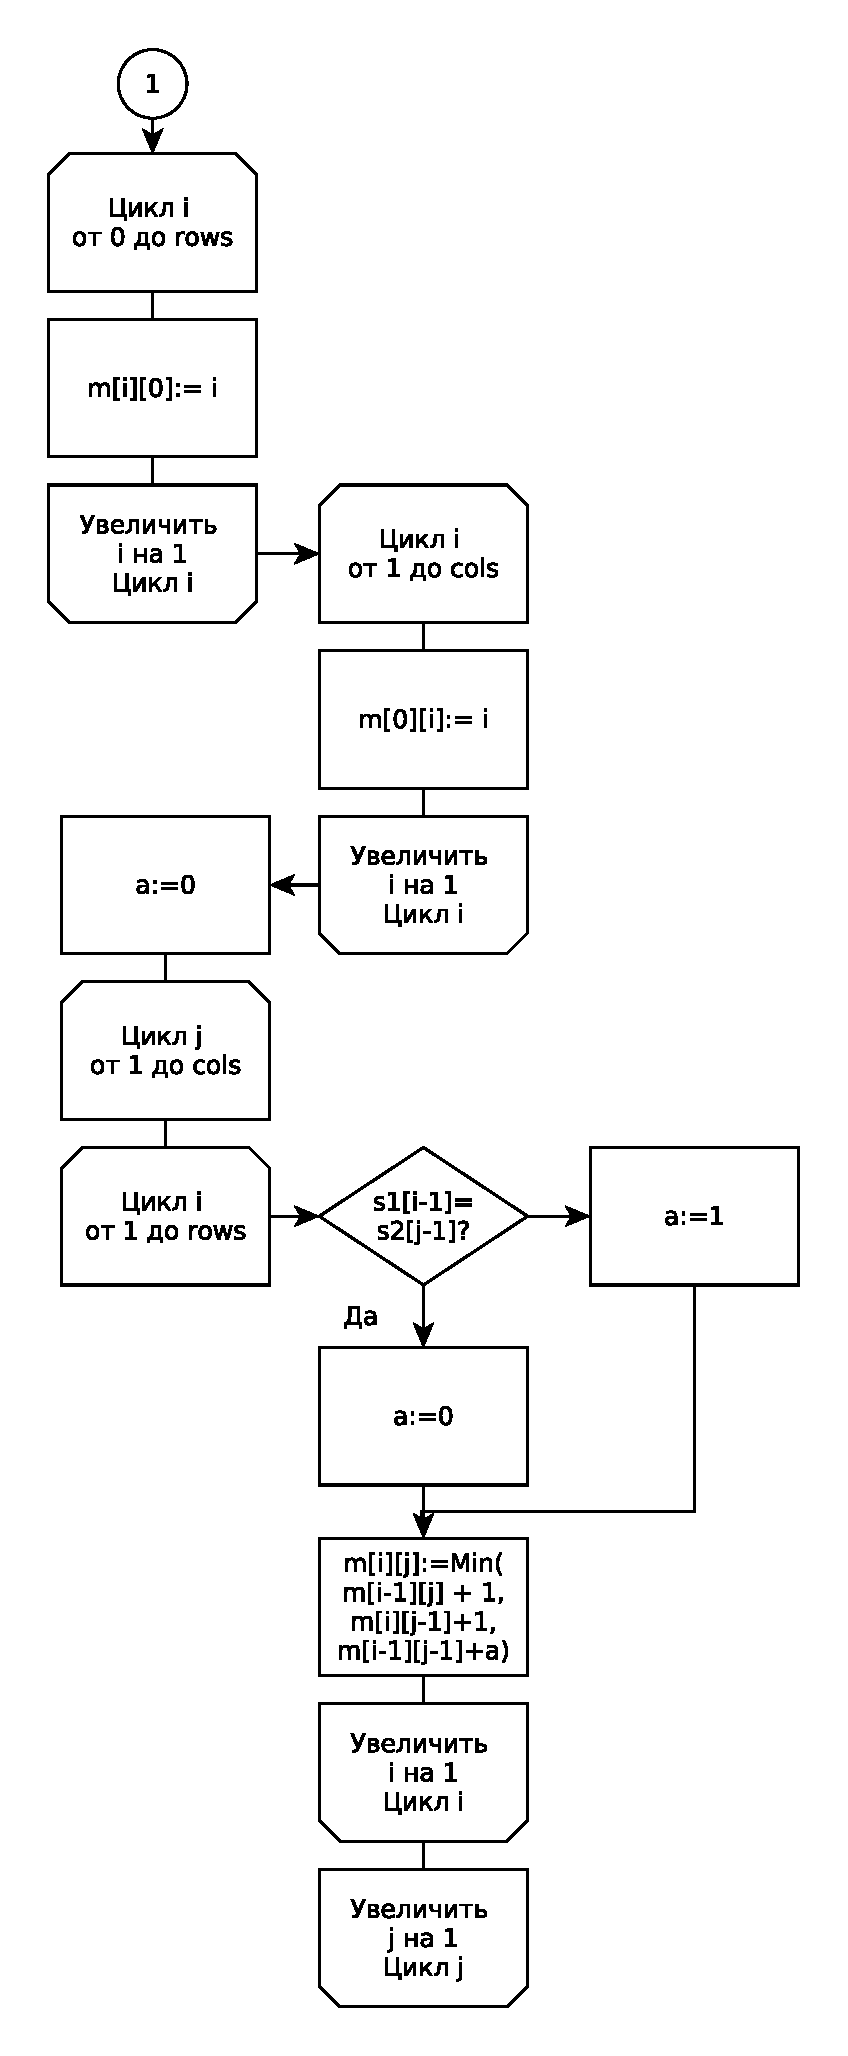
\includegraphics[height=0.75\textheight]{schemes/levenshtein-iterative-eps-2}
    \caption{Схема алгоритма определения расстояния Левенштейна в матричной реализации. Часть 2.}
    \label{levenshtein-iterative-scheme-part-2}
\end{figure}

\FloatBarrier

На рис. \ref{levenshtein-damerau-scheme-part-1} и рис. \ref{levenshtein-damerau-scheme-part-2} представлена схема алгоритма определения расстояния Дамерау-Левенштейна в матричной реализации.

\begin{figure}
    \centering
    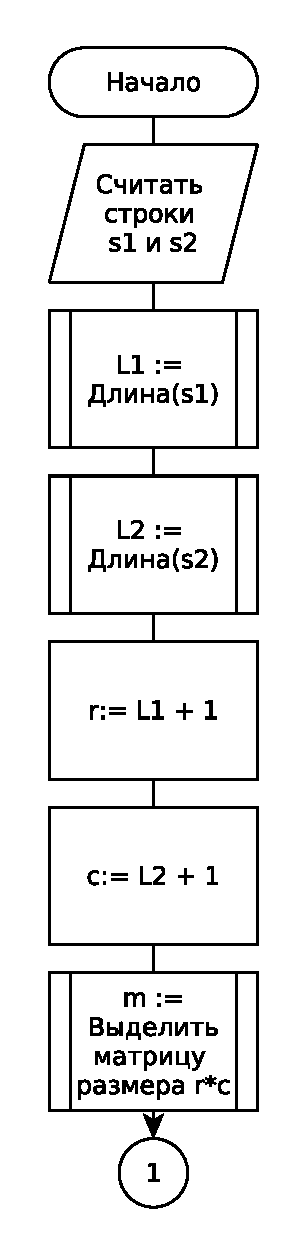
\includegraphics[height=0.75\textheight]{schemes/levenshtein-damerau-eps-1}
    \caption{Схема алгоритма определения расстояния Дамерау-Левенштейна. Часть 1.}
    \label{levenshtein-damerau-scheme-part-1}
\end{figure}

\begin{figure}
    \centering
    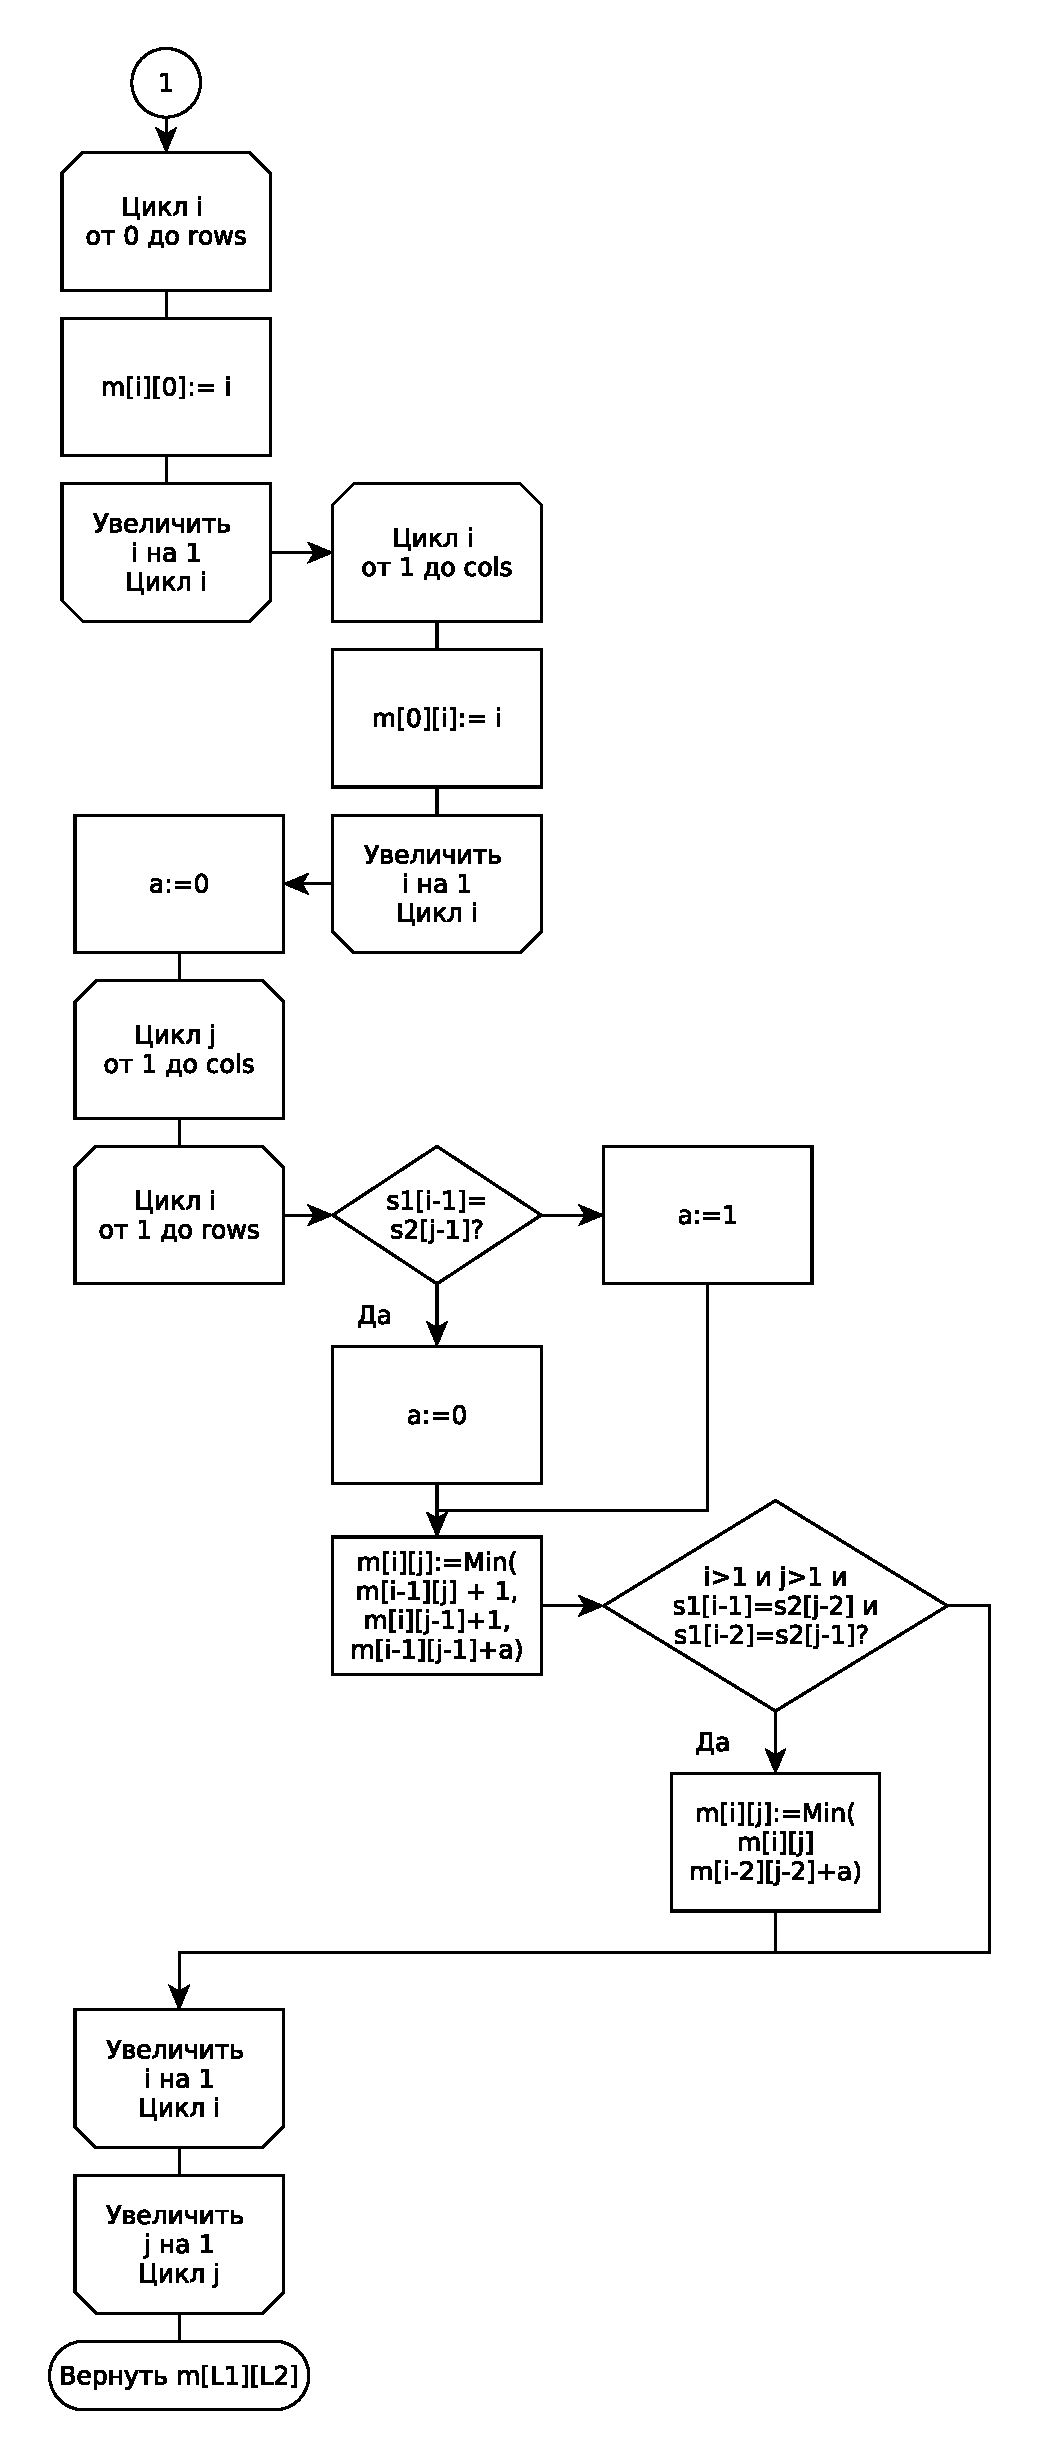
\includegraphics[height=0.75\textheight]{schemes/levenshtein-damerau-eps-2}
    \caption{Схема алгоритма определения расстояния Дамерау-Левенштейна. Часть 2.}
    \label{levenshtein-damerau-scheme-part-2}
\end{figure}

\FloatBarrier

\section{Сравнительный анализ рекурсивной и нерекурсивной\\ реализаций}

Рекурсивная реализация по сравнению с матричной будет иметь большую сложность.
В матричной количество итераций заранее известно и будет равно
$m * n$, где $m$ - число строк, а $n$ -число столбцов.

При этом в рекурсивной версии сложность может достигать $3^{max(m, n)}$, так как
на каждый вызов функции может требоваться ещё 3. При этом в данном дереве рекурсии
на некоторых ветвях будут производится повторные вычисления, что неэффективно.
